\subsection{Model \#1: fixed stars, fixed planets, twin binaries}
\label{sec:model_1}

Since the effects of binarity are most pronounced when the two components are 
similar, we begin by considering a universe in which all planets are 
identical, and all stars are identical except that some fraction of them exist 
in binaries.

Expressed mathematically, from Eqs.~\ref{eq:rate_density_marginalized}
and~\ref{eq:rate_density_shape} the occurrence rate density at a planet radius 
$r$ can be written
\begin{equation}
\Gamma(r) = \delta(r_p) \times
\frac{
    N_0 Z_0 +
    N_1 Z_1 +
    N_2 Z_2
}{N_{\rm tot}},
\label{eq:model_1_rate_density}
\end{equation}
where $\delta(r_p)$ is the Dirac delta function, zero except at the true 
planet radius, $r_p$.
The occurrence rate over any interval that includes $r_p$ is then
\begin{equation}
\Lambda|_{r_p} = \frac{
    N_0 Z_0 +
    N_1 Z_1 +
    N_2 Z_2 
}{N_{\rm tot}},
\label{eq:model_1_rate}
\end{equation}
and the rate is zero over intervals that do not include $r_p$.

We return to our group of binarity-ignoring astronomers. They do 
not know the true rate density~--~they would like to discover it!
In their signal-to-noise limited transit survey, they select stars 
that they think can yield transit detections.
Since the noise is Poissonian, they assume
\begin{equation}
\frac{{\rm signal}}{{\rm noise}}
\propto \frac{(r/R)^2}{F^{-1/2}}
\propto F^{1/2}
\propto L_{\rm sys}^{1/2} d^{-1}, \quad ({\rm incorrectly\ assumed})
\end{equation}
for $R$ the constant stellar radius, $F$ the photon flux, $L_{\rm sys}$ the 
luminosity of a system, and $d$ its distance from us.
At fixed planet radius, semimajor axis, stellar radius, and stellar luminosity,
a constant signal-to-noise floor yields a maximum detectable 
distance~\citep{pepper_using_2003,pepper_searching_2005}.
The maximum distance out to which our binarity-ignoring astronomers 
select stars, $d_{\rm sel}$, thus scales as $L_{\rm sys}^{1/2}$.

The single stars have luminosity $L_1$, and the twin binaries have luminosity 
$2L_1$.
Thus the twin binaries are selected out to a distance $\sqrt{2}$ times 
that of single stars.
This is a bad move, because the transit signal for any planet in a 
twin binary will be diluted by a factor of two:
\begin{equation}
\frac{{\rm signal}}{{\rm noise}}
\propto \frac{\mathcal{D} (r/R)^2}{F^{-1/2}}
\propto \mathcal{D} F^{1/2}
\propto \mathcal{D} L_{\rm sys}^{1/2} d^{-1}, \quad ({\rm true})
\label{eq:snr_true}
\end{equation}
where the dilution is $\mathcal{D} \equiv L_{\rm host}/L_{\rm sys}$, for 
$L_{\rm host}$ the the planet host's luminosity.
This means that the true maximum searchable distance for binaries, $d_{\rm 
det}$, is $1/\sqrt{2}$ times that of single stars.
The situation is illustrated in Fig.~\ref{fig:model_1_volumes}: only one in 
eight selected stars in binaries are truly searchable.

\begin{figure}[!tb]
    \begin{center}
        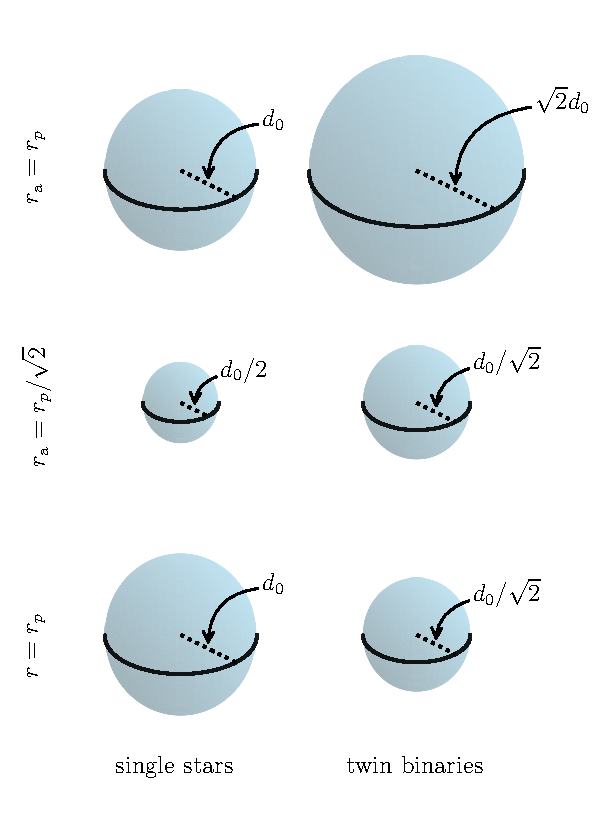
\includegraphics[width=0.6\textwidth]{figures/visualize_volumes.pdf}
    \end{center}
    \caption{
        Cartoon of the searchable volumes for single stars ({\it left}), and 
        twin binaries ({\it right}).
        This model (\#1) assumes all stars have equal mass and luminosity, and 
        all planets have the same true radius $r=r_p$.
        {\it Top:} At an apparent radius $r\a=r_p$,
        the observer selects twin binaries out to a larger         
        distance, $\sqrt{2}\times$ that of single stars.
        Because of dilution, there are no planets in twin binaries with 
        $r\a=r_p$.
        {\it Middle:} At an apparent radius $r\a=r_p/\sqrt{2}$, the 
        searched volumes are half those at $r\a=r_p$. 
        The only detected planets with $r\a=r_p/\sqrt{2}$ orbit twin binaries.
        {\it Bottom:} Planets with a true radius $r=r_p$ are searchable to 
        a maximum distance $d_0$ around singles, and $d_0/\sqrt{2}$ around 
        twin binaries. These distances are the same as what an observer 
        selects based on apparent radii.
    }
    \label{fig:model_1_volumes}
\end{figure}


\paragraph{What do the observers ignoring binarity infer?} 
The binarity-ignoring observers assume that all points on the sky with flux 
above some minimum are searchable.
They correct their assumed number of searchable stars for the transit 
probability.
As a function of apparent radius, they then report an apparent rate density of
\begin{equation}
\Gamma_a(r_a) = 
\delta(r_p) Z_0 \frac{N_0}{N_0+N_1}  +
\delta\left(\frac{r_p}{\sqrt{2}}\right) 
(Z_1 p_{{\rm det},1} + Z_2 p_{{\rm det},2}) \frac{N_1}{N_0+N_1},
\label{eq:model_1_apparent_rate_density}
\end{equation}
where $p_{{\rm det},1}$ ($p_{{\rm det},2}$) is the probability that a selected 
primary (secondary) is searchable.
In this example, $p_{{\rm det},1}=p_{{\rm det},2}=1/8$; the detection 
efficiency is the ratio of the searchable to selected volumes.

The true rate density (Eq.~\ref{eq:model_1_rate_density}) and the
apparent rate density (Eq.~\ref{eq:model_1_apparent_rate_density})
differ in that
\begin{enumerate}
\item The total number of selected stars, $N_{\rm tot} = N_0+N_1+N_2$, was 
miscounted.
%
\item The detection efficiency was incorrectly assumed to be $1$ for all 
selected stars. In reality, only one in eight binaries were searchable.
%
\item The inferred radii in binary systems are all $\sqrt{2}$ too small.
\end{enumerate}

To assess the severity of these errors, we need to make assumptions about the 
stellar and planetary populations.
The important quantity for the stellar population is $N_1/N_0$, the ratio of 
selected primaries (or binaries) to singles. We can define
\begin{align}
\mu \equiv \frac{N_1}{N_0} &=
\frac{n_b}{n_s} \left(\frac{d_{\rm sel,b}}{d_{\rm sel,s}}\right)^3 = 
\frac{{\rm BF}}{1-{\rm BF}} (1+\ell)^{3/2},
\label{eq:mu_definition}
\end{align}
where $n_b$ and $n_s$ are the number density of binaries and singles in a 
volume limited sample, and the maximum selected distance for binary and single 
systems are $d_{\rm sel,b}$ and $d_{\rm sel,s}$.
The light ratio $\ell$ is defined relative to the primary, so that
$L_{\rm sys} = L_1(1+\ell)$.
The binary fraction in a volume limited sample is ``{\rm BF}''.
For instance, \citet{raghavan_survey_2010} found a multiplicity 
fraction\footnote{
    The binary fraction is the fraction of systems in a volume-limited sample 
    that are binary. It is equivalent to the multiplicity fraction if there 
    are no triple, quadruple, or higher order multiples. In that case, ${\rm 
        BF} = n_b / (n_s+n_b)$.
} of 0.44 for primaries with masses from $0.7M_\odot$ to $1.3M_\odot$. 
``Twin binaries'' are perhaps 10-20\% of the binaries in a volume-limited 
sample, depending on how ``twin'' is defined.
Thus a representative twin binary fraction for this model is ${\rm BF}\approx 
0.05$-$0.1$. 

Further, we need to assume knowledge of the true number of planets per 
single, primary, and secondary star ($Z_0,Z_1,$ and $Z_2$).
Taking $Z_0=Z_1=Z_2=1/2$, we plot the resulting occurrence rates as a function 
of planet radius in Fig.~\ref{fig:errcases_model_1}.
Though it is impossible for an observer to isolate any one of binarity's 
biases without also addressing the others, mathematically it is simply a 
matter of modifying the appropriate terms in 
Eq.~\ref{eq:model_1_apparent_rate_density}.
The resulting rates are also shown in 
Fig.~\ref{fig:errcases_model_1}, and demonstrate how each 
error individually affects the overall inferred rate.

\begin{figure}[!tb]
    \begin{center}
        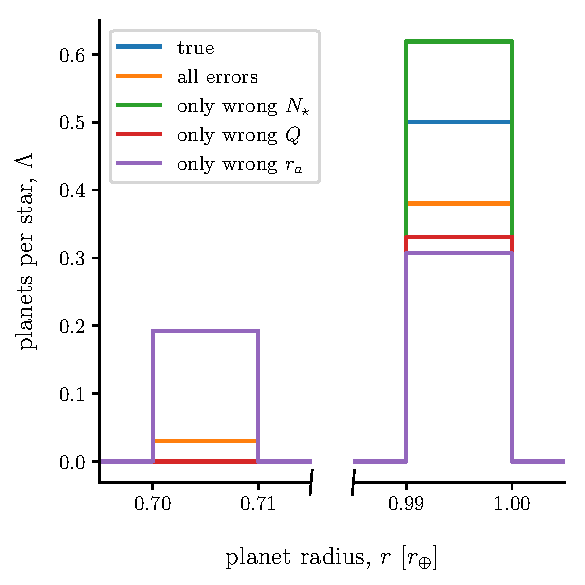
\includegraphics[width=.6\textwidth]{figures/errcases_rate_density_vs_radius_model_1_brokenx.pdf}
    \end{center}
    \vspace{-0.5cm}
    \caption{
        Inferred planet occurrence rates over $0.01r_\oplus$ bins in planet 
        radius,
        for Model \#1.
        This model has fixed stars, fixed planets, and twin binaries. 
        It assumes a twin binary fraction of ${\rm BF}=0.1$.
        If the true planet radius is $r_p$, all planets 
        detected in binaries will have apparent radii $r_a = r_p/\sqrt{2}$.
        We illustrate the individual biases by separating them.
        On this and future plots,
        ``only wrong $N_\star$'' means the only error is an incorrectly 
        assumed 
        number of selected stars;
        ``only wrong $Q$'' means the only error is an incorrectly assumed 
        completeness (including both miscalculated $p_{\rm tra}$ 
        and fraction of selected stars that are searchable, $p_{\rm det}$);
        ``only wrong $r_a$'' means the only error is in miscalculated        
        planetary radii, due to both transit depth dilution and also wrongly 
        assumed host star radii.
    }
    \label{fig:errcases_model_1}
\end{figure}


\paragraph{Correction to inferred rate density and inferred rate}

We define a rate density correction factor, $X_\Gamma$, as the ratio of the 
apparent to true rate densities:
\begin{equation}
X_\Gamma \equiv \frac{\Gamma_a}{\Gamma}.
\end{equation}
This correction factor can be a function of whatever parameters $\Gamma_a$ and 
$\Gamma$ depend on; in this study, the planet radius is most relevant.

If we continue assuming that the number of planets per single, primary, and 
secondary star are equal ($Z_0=Z_1=Z_2$), we find a rate density correction 
factor at the true planet radius of
\begin{equation}
X_\Gamma(r_p) = \frac{1}{1+\mu},
\label{eq:Z_eq_model_1_correction}
\end{equation}
This yields a correction of 0.76 if ${\rm BF}=0.1$, and 0.87 if ${\rm 
BF}=0.05$.
Rephrasing the result, if the twin binary fraction were 
$(2^{3/2}+1)^{-1}\approx 0.26$, then the apparent rate would be half the true 
rate.
Fortunately, in most contexts the twin binary fraction is not that high.

An alternative assumption is that secondaries do not host planets. In that 
case, $Z_0=Z_1$, and $Z_2=0$. The correction to the rate density at the true 
planet radius becomes
\begin{equation}
X_\Gamma(r_p) = \frac{1+2\mu}{(1+\mu)^2}.
\end{equation}
This evaluates to 0.94 if ${\rm BF}=0.1$, and 0.98 if ${\rm BF}=0.05$.
While it is hard to justify the assumption that secondaries are planet-less, 
it is worth noting that $\Gamma_a/\Gamma$ is sensitive to the relative number 
of planets per single, primary, and secondary.